\section{MAGE: \mask-Guided Sparse Attention}
\label{sec:method}


% \begin{algorithm}[t!]
% \small
% \caption{MAGE Inference}
% \label{alg:mage}
% \begin{algorithmic}[1]
% \Require KV cache $\mathcal{C}$, block size $B$, budget $K$, steps $T$
% \Ensure Generated block $\mathbf{x}$

% \State Initialize block with $B$ \texttt{[MASK]} tokens

% \Statex \hspace{-1em} \textit{\textcolor{gray}{// Phase 1: Exact Attention with Union Formation ($t=1$)}}
% \For{each layer $\ell \geq 2$}
%     \State $\mathbf{A}_{\ell} \gets \text{Softmax}(\mathbf{Q}_{\texttt{MASK}} \mathbf{K}^\top / \sqrt{d})$
%     \For{each KV head $h$}
%         \State $\mathcal{T}_q \gets \text{TopK}(\mathbf{A}_\ell[q,:], K)$ for each query $q$
%         \State $\mathcal{U}_h \gets \bigcup_q \mathcal{T}_q$ \Comment{Union via voting}
%         \State $p_h \gets \frac{1}{GB}\sum_q \sum_{i \in \mathcal{U}_h} \mathbf{A}_\ell[q, i]$ \Comment{Coverage}
%     \EndFor
%     \State $s_\ell \gets \max_h |\mathcal{U}_h| \cdot (1 - \log p_h)$ \Comment{Adjusted score}
% \EndFor

% \Statex \hspace{-1em} \textit{\textcolor{gray}{// Phase 2: Index Selection}}
% \For{each layer $\ell$, each KV head $h$}
%     \State $K^\ell \gets \max\left(K_{\min}, \lfloor \frac{s_\ell}{\sum_{\ell'} s_{\ell'}} \cdot K \cdot L \rfloor\right)$
%     \State $\mathbf{T}_{\ell,h} \gets \text{SelectTopK}(\mathcal{U}_h, K^\ell)$ \Comment{From union}
% \EndFor

% \Statex \hspace{-1em} \textit{\textcolor{gray}{// Phase 3: Sparse Denoising ($t=2$ to $T$)}}
% \For{$t = 2$ to $T$}
%     \For{each layer $\ell \geq 2$}
%         \State $\mathbf{o}_{\ell} \gets \text{SparseAttn}(\mathbf{Q}, \mathcal{C}[\mathbf{T}_{\ell}])$
%     \EndFor
%     \State Unmask high-confidence positions
% \EndFor
% \State $\mathcal{C} \leftarrow \mathcal{C} \,\Vert\, \text{KV}(\mathbf{x})$ \Comment{Update KV cache}
% \State \Return $\mathbf{x}$
% \end{algorithmic}
% \end{algorithm}



\begin{algorithm}[t!]
\small
\caption{MAGE Inference}
\label{alg:mage}
\begin{algorithmic}[1]
\REQUIRE KV cache $\mathcal{C}$, block size $B$, budget $K$, steps $T$
\ENSURE Generated block $\mathbf{x}$
\STATE Initialize block with $B$ \texttt{[MASK]} tokens
\STATE \textit{\textcolor{gray}{// Phase 1: Exact Attention with Union Formation ($t=1$)}}
\FOR{each layer $\ell \geq 2$}
    \STATE $\mathbf{A}_{\ell} \gets \text{Softmax}(\mathbf{Q}_{\texttt{MASK}} \mathbf{K}^\top / \sqrt{d})$
    \FOR{each KV head $h$}
        \STATE $\mathcal{T}_q \gets \text{TopK}(\mathbf{A}_\ell[q,:], K)$ for each query $q$
        \STATE $\mathcal{U}_h \gets \bigcup_q \mathcal{T}_q$ \COMMENT{Union via voting}
        \STATE $p_h \gets \frac{1}{GB}\sum_q \sum_{i \in \mathcal{U}_h} \mathbf{A}_\ell[q, i]$ \COMMENT{Coverage}
    \ENDFOR
    \STATE $s_\ell \gets \max_h |\mathcal{U}_h| \cdot (1 - \log p_h)$ \COMMENT{Adjusted score}
\ENDFOR
\STATE \textit{\textcolor{gray}{// Phase 2: Index Selection}}
\FOR{each layer $\ell$, each KV head $h$}
    \STATE $K^\ell \gets \max\left(K_{\min}, \lfloor \frac{s_\ell}{\sum_{\ell'} s_{\ell'}} \cdot K \cdot L \rfloor\right)$
    \STATE $\mathbf{T}_{\ell,h} \gets \text{SelectTopK}(\mathcal{U}_h, K^\ell)$ \COMMENT{From union}
\ENDFOR
\STATE \textit{\textcolor{gray}{// Phase 3: Sparse Denoising ($t=2$ to $T$)}}
\FOR{$t = 2$ to $T$}
    \FOR{each layer $\ell \geq 2$}
        \STATE $\mathbf{o}_{\ell} \gets \text{SparseAttn}(\mathbf{Q}, \mathcal{C}[\mathbf{T}_{\ell}])$
    \ENDFOR
    \STATE Unmask high-confidence positions
\ENDFOR
\STATE $\mathcal{C} \leftarrow \mathcal{C} \,\Vert\, \text{KV}(\mathbf{x})$ \COMMENT{Update KV cache}
\STATE \textbf{return} $\mathbf{x}$
\end{algorithmic}
\end{algorithm}


Based on the observations in Section 3, we propose MAGE ([MASK]-Guided Sparse Attention), a dynamic sparse attention method that uses the attention scores computed on the first denoising step's All-[MASK] block to guide the remaining steps of block generation.




\subsection{MAGE Inference}
\label{subsec:mage_inference}

Algorithm~\ref{alg:mage} presents the complete MAGE inference procedure. For each block, the first denoising step computes exact attention on the All-\mask block and selects critical KV indices with layer-adaptive budgets. All subsequent steps reuse these selected indices for sparse attention.



\paragraph{Phase 1: Exact Attention with Union Formation.}
In the first denoising step, we compute exact attention between the All-\mask block and all preceding KV cache, obtaining the attention matrix $\mathbf{A}_\ell$ for each layer $\ell$.
For each query $q$, we select its local top-$K$ indices based on the attention scores.
These selections are aggregated across all $G \times B$ queries sharing each KV head $h$ by taking their union, forming a head-specific set $\mathcal{U}_h$ that covers the top-$K$ indices of all queries.
To quantify attention coverage for each KV head, we compute the coverage $p_h$, the average attention probability captured by the union: 

\begin{equation}
p_h = \frac{1}{GB}\sum_{q} \sum_{i \in \mathcal{U}_h} \mathbf{A}[q, i]
\end{equation}
Not all layers require the same number of KV entries: layers where attention is concentrated on a few positions can operate with a smaller allocation, while layers with dispersed attention need more.
To estimate each layer's demand, we define an \textit{adjusted score} $s_{\ell,h}$ per KV head that combines union size with attention coverage:
\begin{equation}
s_{\ell,h} = |\mathcal{U}_h| \cdot (1 - \log p_h)
\end{equation}
A larger union or lower coverage both increase the score, indicating that the head requires more KV entries. We take the maximum across heads as the layer's adjusted score $s_\ell = \max_h s_{\ell,h}$, since all heads within a layer share the same allocation in practice for memory access efficiency.

\begin{figure*}[t!]
    \centering
    % \includegraphics[width=\linewidth]
    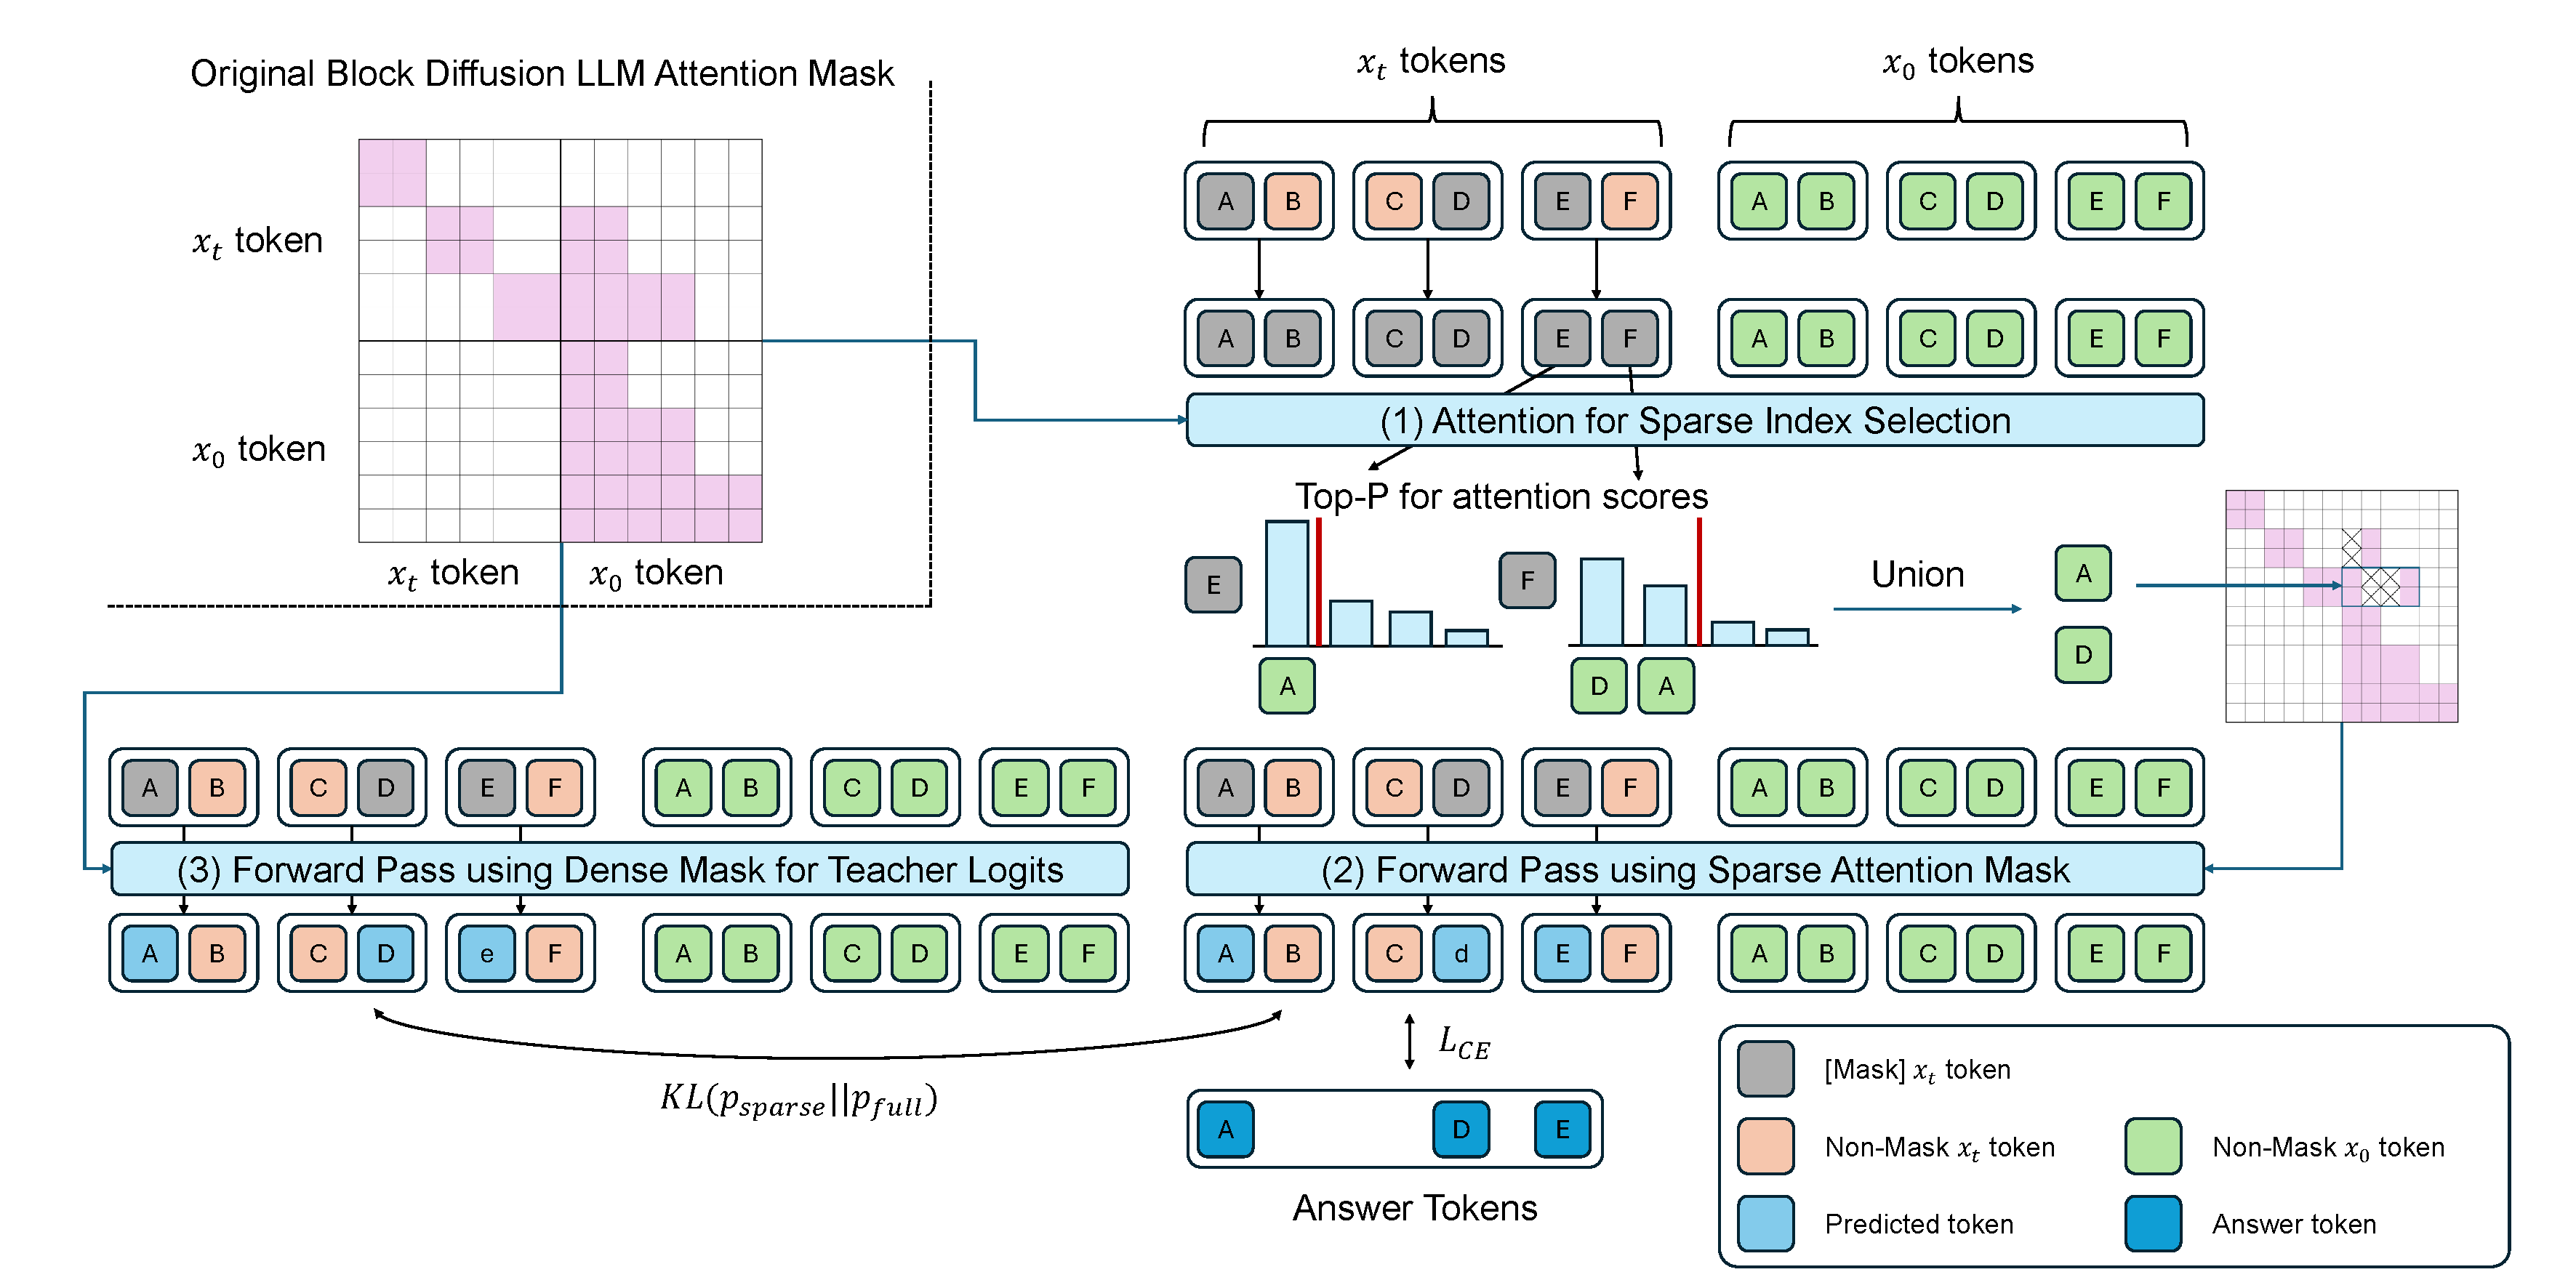
\includegraphics[width=\textwidth]
    {figures/fig8_finetune.pdf}
    \caption{Overview of the MAGE Fine-tuning process. The process consists of three stages: (1) Index Selection identifies important KV indices via Top-K selection without gradients; (2) Sparse Forward applies the sparse mask and computes gradients; (3) Teacher Forward provides exact reference logits for self-distillation.}
    \label{fig:finetuning}
\end{figure*}



\paragraph{Phase 2: Layer-Adaptive Allocation and Selection.}
Given a target budget $K$ per layer on average, MAGE distributes the total budget $K \times L$ proportionally based on adjusted scores:
\begin{equation}
K^\ell = \max\left(K_{\min}, \left\lfloor \frac{s_\ell}{\sum_{\ell'} s_{\ell'}} \cdot K \cdot L \right\rfloor\right)
\end{equation}
where $K_{\min}$ ensures a minimum allocation per layer. Each KV head constructs its final index set $\mathbf{T}_{\ell,h}$ by selecting top-$K^\ell$ indices from the union based on voting scores. If the allocation exceeds the union size, the entire union is included and remaining slots are filled with recent KV positions.
Notably, since index selection for layer $\ell$ 
depends only on statistics computed at layer $\ell$, it can be overlapped with the exact attention computation of layer $(\ell+1)$, effectively hiding the overhead.
In contrast, Quest must complete importance estimation before attention can proceed, and Tidal requires the previous layer's results, making their overhead unavoidable. We provide detailed latency analysis in Section~\ref{subsec:efficiency}.

\begin{figure*}[t!]
    \centering
    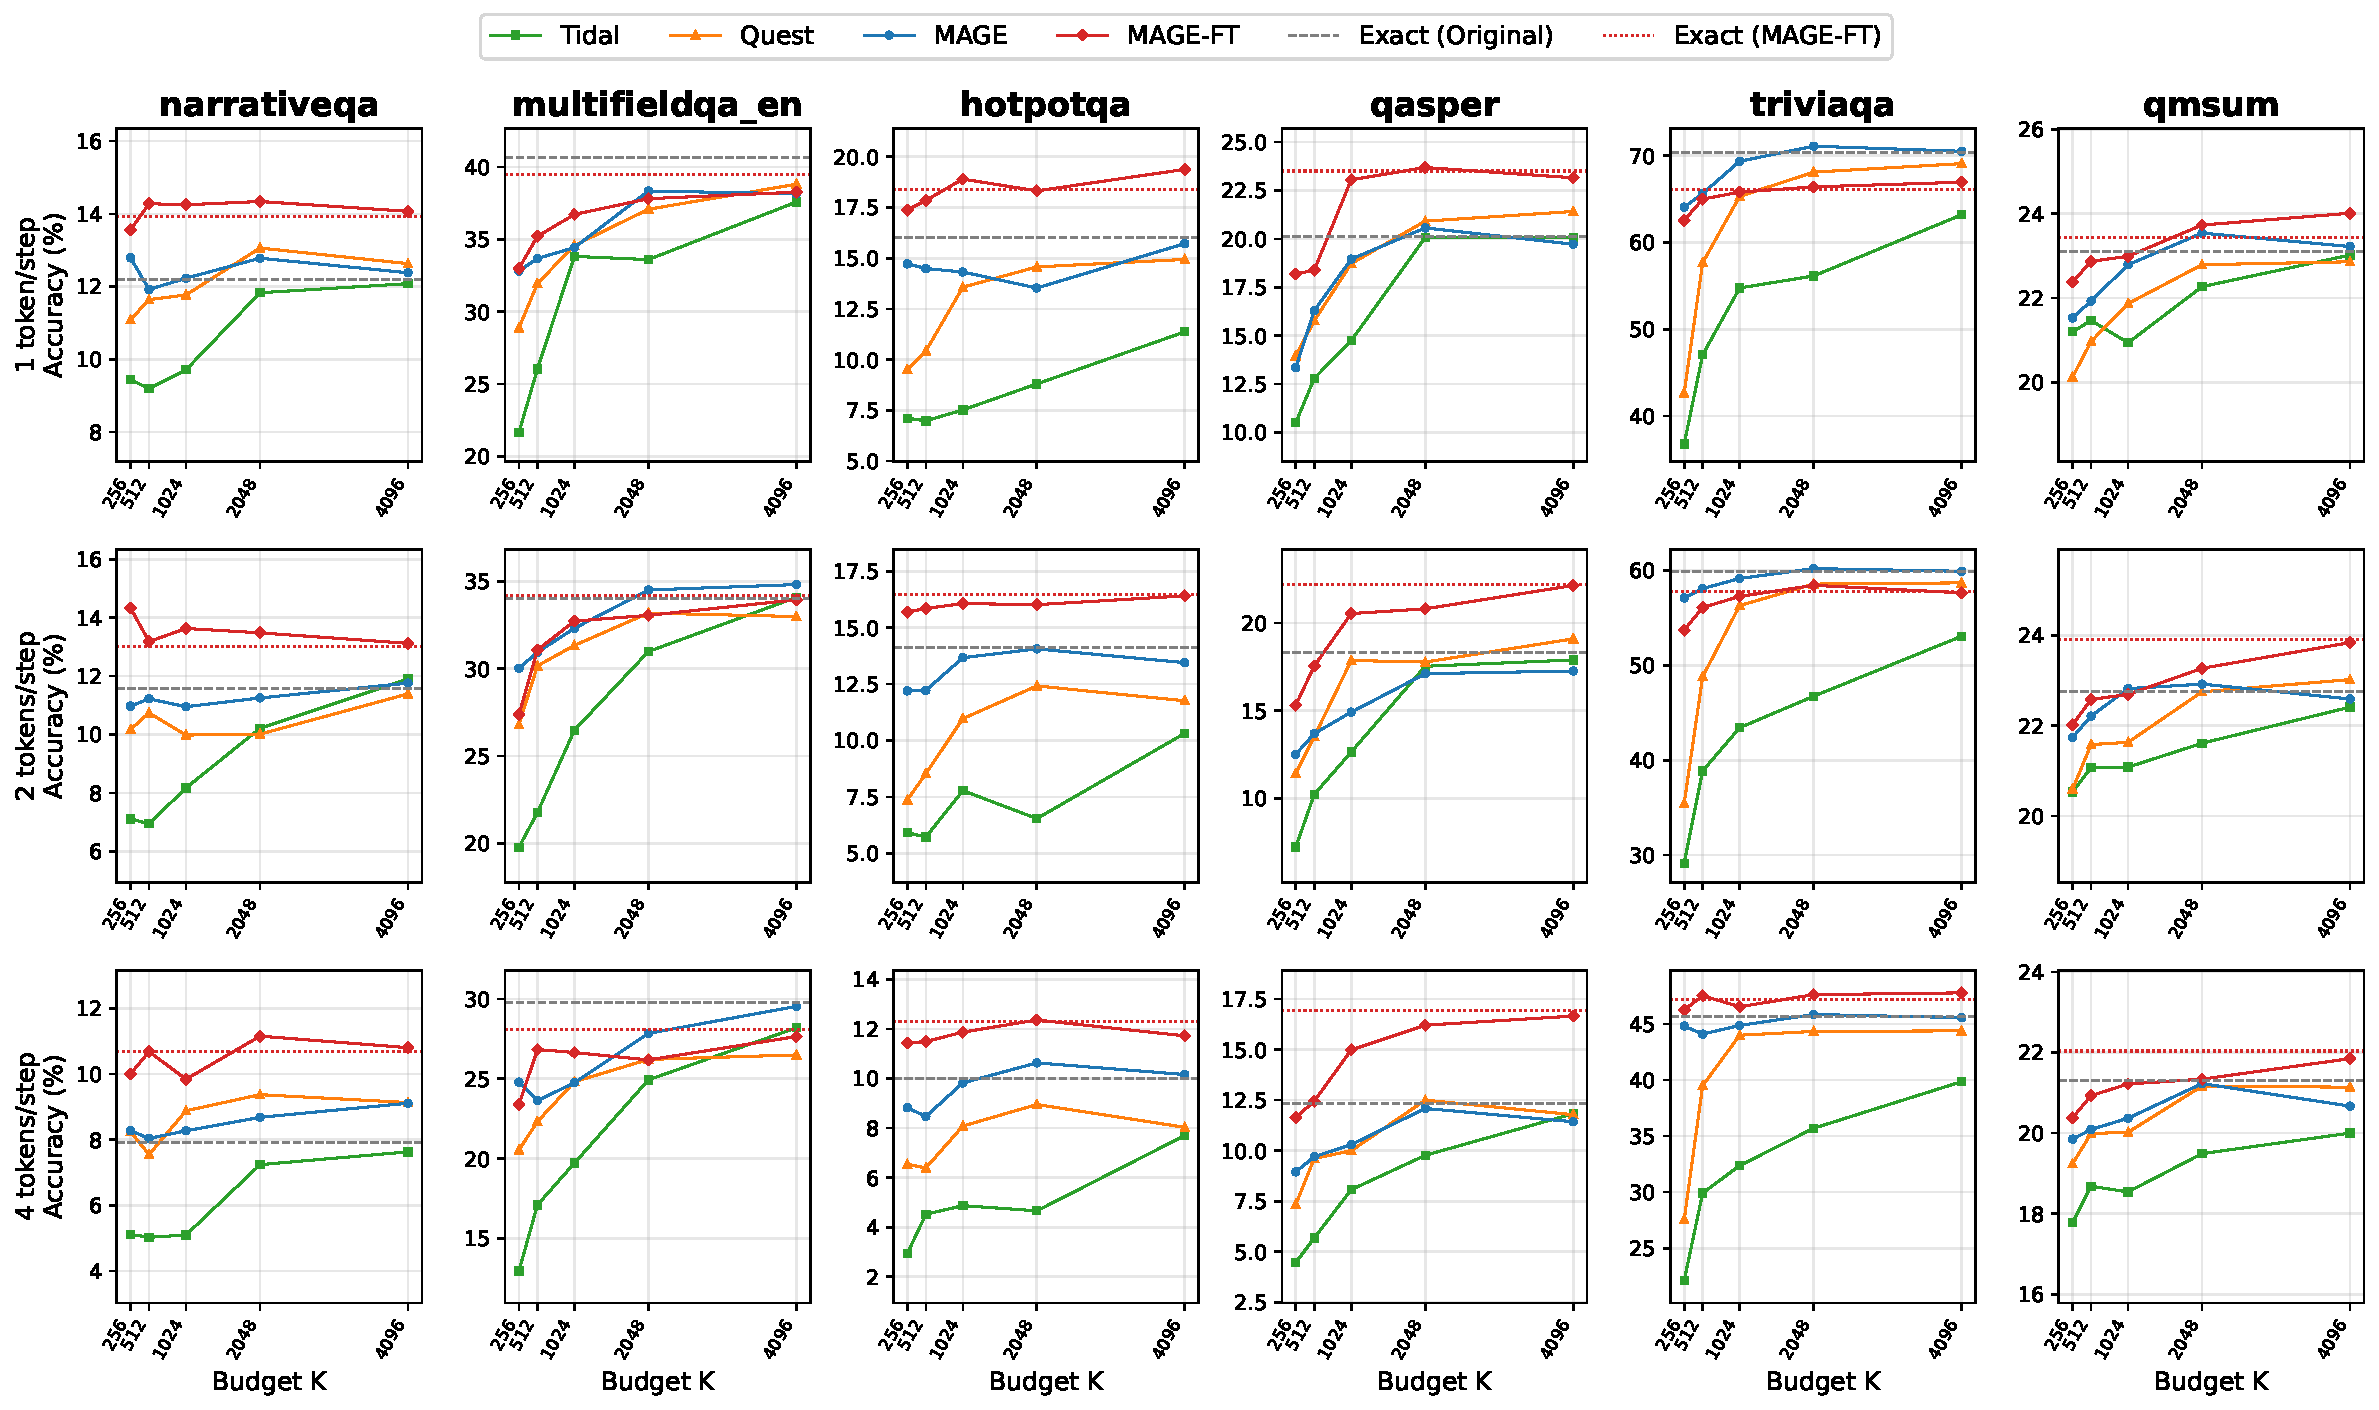
\includegraphics[width=\textwidth]{figures/fig5_1.5b_acc_static_combined.pdf}
    \caption{Per-task accuracy on LongBench with Fast-dLLM 1.5B across three denoising configurations (1, 2, 4 tokens/step). MAGE and MAGE-FT consistently outperform Quest and Tidal across all tasks and budgets. MAGE-FT often surpasses exact attention at moderate budgets, while maintaining robustness at higher tokens per step.}
    \label{fig:longbench_accuracy}
\end{figure*}


\paragraph{Phase 3: Sparse Denoising.}
The selected indices $\mathbf{T}_{\ell,h}$ are cached and reused for all subsequent denoising steps ($t = 2$ to $T$). At each step, sparse attention retrieves only the KV pairs at these positions, and the model progressively unmasks high-confidence tokens. This reuse is justified by our observation that \mask-identified critical positions remain consistent throughout denoising.


\subsection{Fine-tuning for Boosting All-\mask Block's Guidance}
\label{subsec:fine_tuning}



While \name works effectively without training, lightweight fine-tuning can further improve sparse attention accuracy by encouraging the model to more consistently attend to relevant context in the All-\mask block state.
To achieve this, we design a three-stage training process (Figure~\ref{fig:finetuning}) that aligns the model with \name's inference scheme.
Following Fast-dLLM-v2~\citep{wu2025fastdllmv2}, we duplicate each training sample into a noisy half $x_t$, where a subset of tokens in each block is randomly replaced with \mask tokens, and a clean half $x_0$ containing the original uncorrupted text.
We apply an offset block-causal mask that restricts queries from $x_t$ to attend only to their corresponding $x_0$ blocks.


\paragraph{Forward Process.}
Figure~\ref{fig:finetuning} illustrates the three stages.
\textit{Stage 1: Sparse Index Selection.}
Mirroring MAGE inference, we compute exact attention on the All-\mask block ($x_t$ replaced with \mask tokens) and select critical KV indices via Top-P on the attention scores.
This pass runs without gradient computation.
We take the union of selected indices across all query heads sharing the same KV head and cache them for the subsequent stage.

\textit{Stage 2: Sparse-Aware Forward.}
We execute the primary gradient-based forward pass using the cached sparse indices.
The sparse mask is applied specifically to the cross-attention region ($x_t \to x_0$), while self-attention within the context ($x_0 \to x_0$) and within the noisy block ($x_t \to x_t$) remains exact.
To ensure training stability, the initial two layers maintain exact attention.

\textit{Stage 3: Teacher Forward.}
We perform an inference-only pass using exact attention to generate reference teacher logits for self-distillation.



\paragraph{Training Objective.}
We employ self-distillation where the same model serves as both teacher and student.
We observe that optimizing with cross-entropy loss alone provides insufficient signal for for adapting the model under sparse attention; thus we introduce KL divergence loss to encourage the sparse-constrained model to mimic the exact teacher's outputs:
\begin{equation}
\mathcal{L} = \mathcal{L}_{\text{CE}} + \lambda\,\text{KL}(p_{\text{sparse}} \| p_{\text{exact}})
\end{equation}
where $\mathcal{L}_{\text{CE}}$ is the cross-entropy loss with ground truth tokens, and $p_{\text{exact}}$, $p_{\text{sparse}}$ are softmax distributions (with temperature $\tau$) from exact and sparse attention paths respectively. Gradients flow only through $p_{\text{sparse}}$; the exact path serves as a fixed target.

\paragraph{Fine-tuning Time.}
Although this scheme requires three forward passes, the overhead is significantly mitigated as two passes (Stages 1 and 3) are executed without gradient tracking. Our approach achieves strong 
sparse accuracy within 200 steps for Fast-dLLM 1.5B  and 100 steps for Fast-dLLM 7B on a single NVIDIA H100 GPU.

